% !TEX encoding = UTF-8
% !TEX TS-program = pdflatex
% !TEX root = ../../tesi.tex

\section{Processi aziendali}
Sync Lab conta di raggiungere i propri obiettivi aziendali attraverso i processi spiegati di seguito.

\subsection{Consulenza}

\begin{figure}[!h]
  \centering
  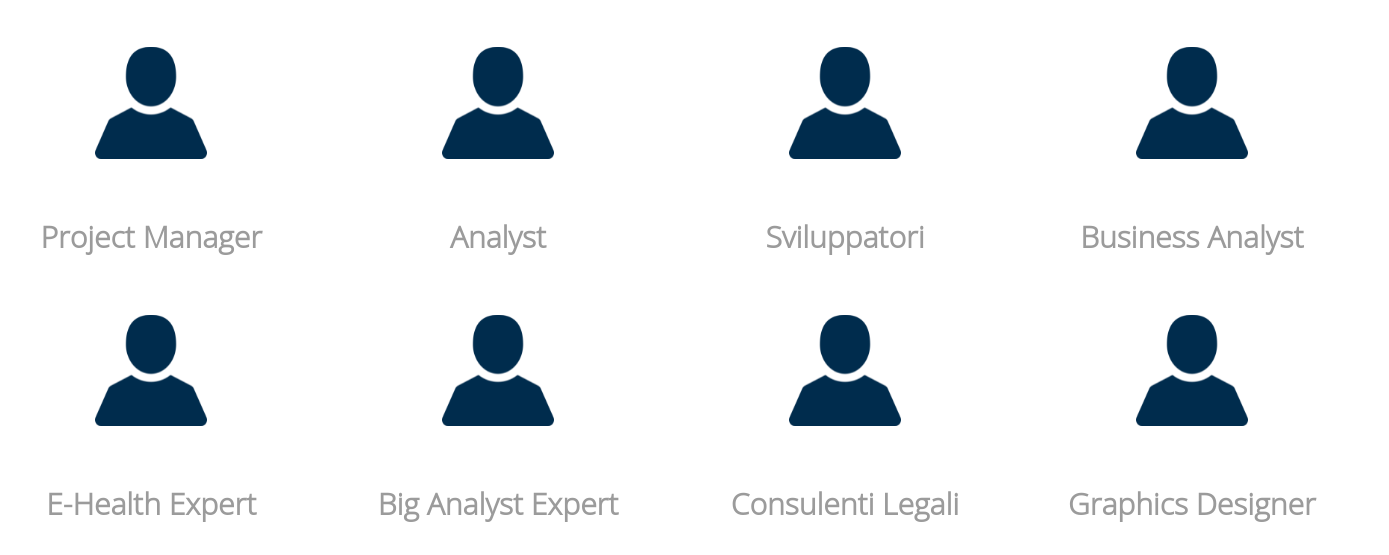
\includegraphics[width=\textwidth]{capitolo1/profili-professionali.png}
  \caption{I profili professionali messi a disposizione da Sync Lab}
  \textbf{Fonte}: \href{https://www.synclab.it/servizi-professionali.php}{https://www.synclab.it/servizi-professionali.php}
\end{figure}

In quanto \textit{partner} di grandi imprese italiane, come spiegato nella sezione precedente, uno degli obiettivi principali di Sync Lab è quello di fornire una consulenza ai suoi clienti che porti un'evoluzione in termini di competitività, sviluppo e innovazione tecnologica. Inoltre, mette a disposizione un team di grande esperienza che interviene nella progettazione e realizzazione delle strategie necessari alla realizzazione di grandi progetti.

\subsection{Fornitura}
La procedura di fornitura viene avviata ogni qual volta che un cliente incarica Sync Lab per la realizzazione di un prodotto. Parallelamente, mette in atto le seguenti attività con lo scopo di migliorare questo processo:
\begin{itemize}
  \item \textbf{Miglioramento delle performance}: verifica e correzione, se necessario, delle procedure aziendali utilizzando le giuste metodologie (\textit{best practices});
  \item \textbf{Ottimizzazione della qualità}: utilizzo di \textit{design patterns} adatti al contesto aziendale;
  \item \textbf{Sviluppo delle quote di mercato}: analisi e miglioramento degli standard di qualità presso l'azienda.
\end{itemize} 

\subsection{Sviluppo}
Sync Lab fa ampio uso del modello di sviluppo Agile, più in particolare della metodologia Scrum, per permettere agli \textit{stakeholders} di seguire l'evoluzione dello sviluppo del prodotto richiesto, raccogliendo tutti i \textit{feedback} che possono essere determinanti per la loro soddisfazione. 

\paragraph{La metodologia Scrum}
Scrum è la metodologia Agile più diffusa tra i team di sviluppo. In questa metodologia gli \textit{stakeholders} hanno un ruolo fondamentale e la loro soddisfazione è determinante per la buona riuscita del progetto. Per rispondere al meglio a questa esigenza, si basa su tre pilastri fondamentali:
\begin{enumerate}
  \item \textbf{Trasparenza}: tutti coloro che partecipano ad un progetto sanno qual è lo scopo (trasparenza verticale) e sanno che cosa fanno gli altri (trasparenza orizzontale). In più, anche lo stato del progetto, con le relative statistiche, è visibile a tutti a prescindere dal livello organizzativo;
  \item \textbf{Ispezione}: ogni iterazione ed incremento vengono verificati in base alle metriche di misurazione decise, in modo tale da modificare le iterazioni successive e rendere così estremamente adattabile l'andamento del processo;
  \item \textbf{Adattamento}: è la conseguenza dell'ispezione e significa che al posto di seguire un piano preordinato, il team di sviluppo pianifica in base ai risultati dell'ispezione per apportare il maggior valore al cliente finale.
\end{enumerate}

\clearpage

\begin{figure}[h!]
  \centering
  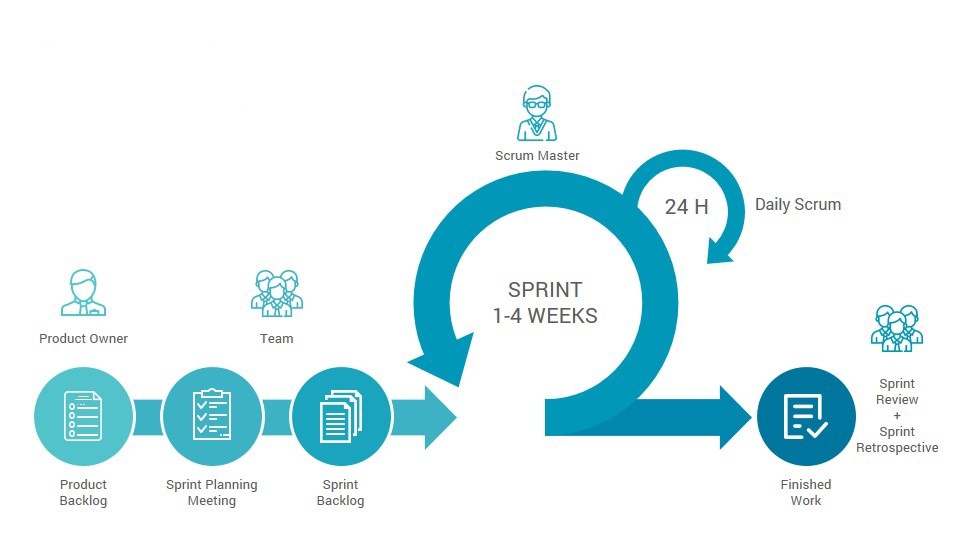
\includegraphics[width=0.8\textwidth]{capitolo1/scrum.jpeg}
  \caption{La metodologia Scrum}
  \textbf{Fonte}: \href{https://medium.com/swlh/agile-primer-for-non-technical-teams-1deb06968281}{https://medium.com/swlh/agile-primer-for-non-technical-teams}
\end{figure}

Durante il periodo di stage ho potuto osservare come vengono organizzati e gestiti i vari \textit{sprint} in Sync Lab. Ad ogni \textit{sprint} corrisponde l'introduzione di una nuova funzionalità che viene opportunamente verificata e comprovata dalla soddisfazione del cliente. L'esecuzione di uno \textit{sprint} prevederà i seguenti passi:
\begin{enumerate}
  \item si definisce un \textbf{\textit{product backlog}}, dove verranno riportate le attività da fare in una \textit{scrum board}, relative al progetto;
  \item si realizza uno \textbf{\textit{sprint planning}}, un sottoinsieme di obiettivi da raggiungere durante un singolo \textit{sprint} sulla base del \textit{product backlog};
  \item si esegue lo \textbf{\textit{sprint}} in un lasso di tempo limitato di massimo 4 settimane;
  \item si revisiona lo \textbf{\textit{sprint goal}} in cui si valuta l'incremento effettivo al termine dello \textit{sprint}.
\end{enumerate}

% \clearpage

\begin{figure}[h!]
  \centering
  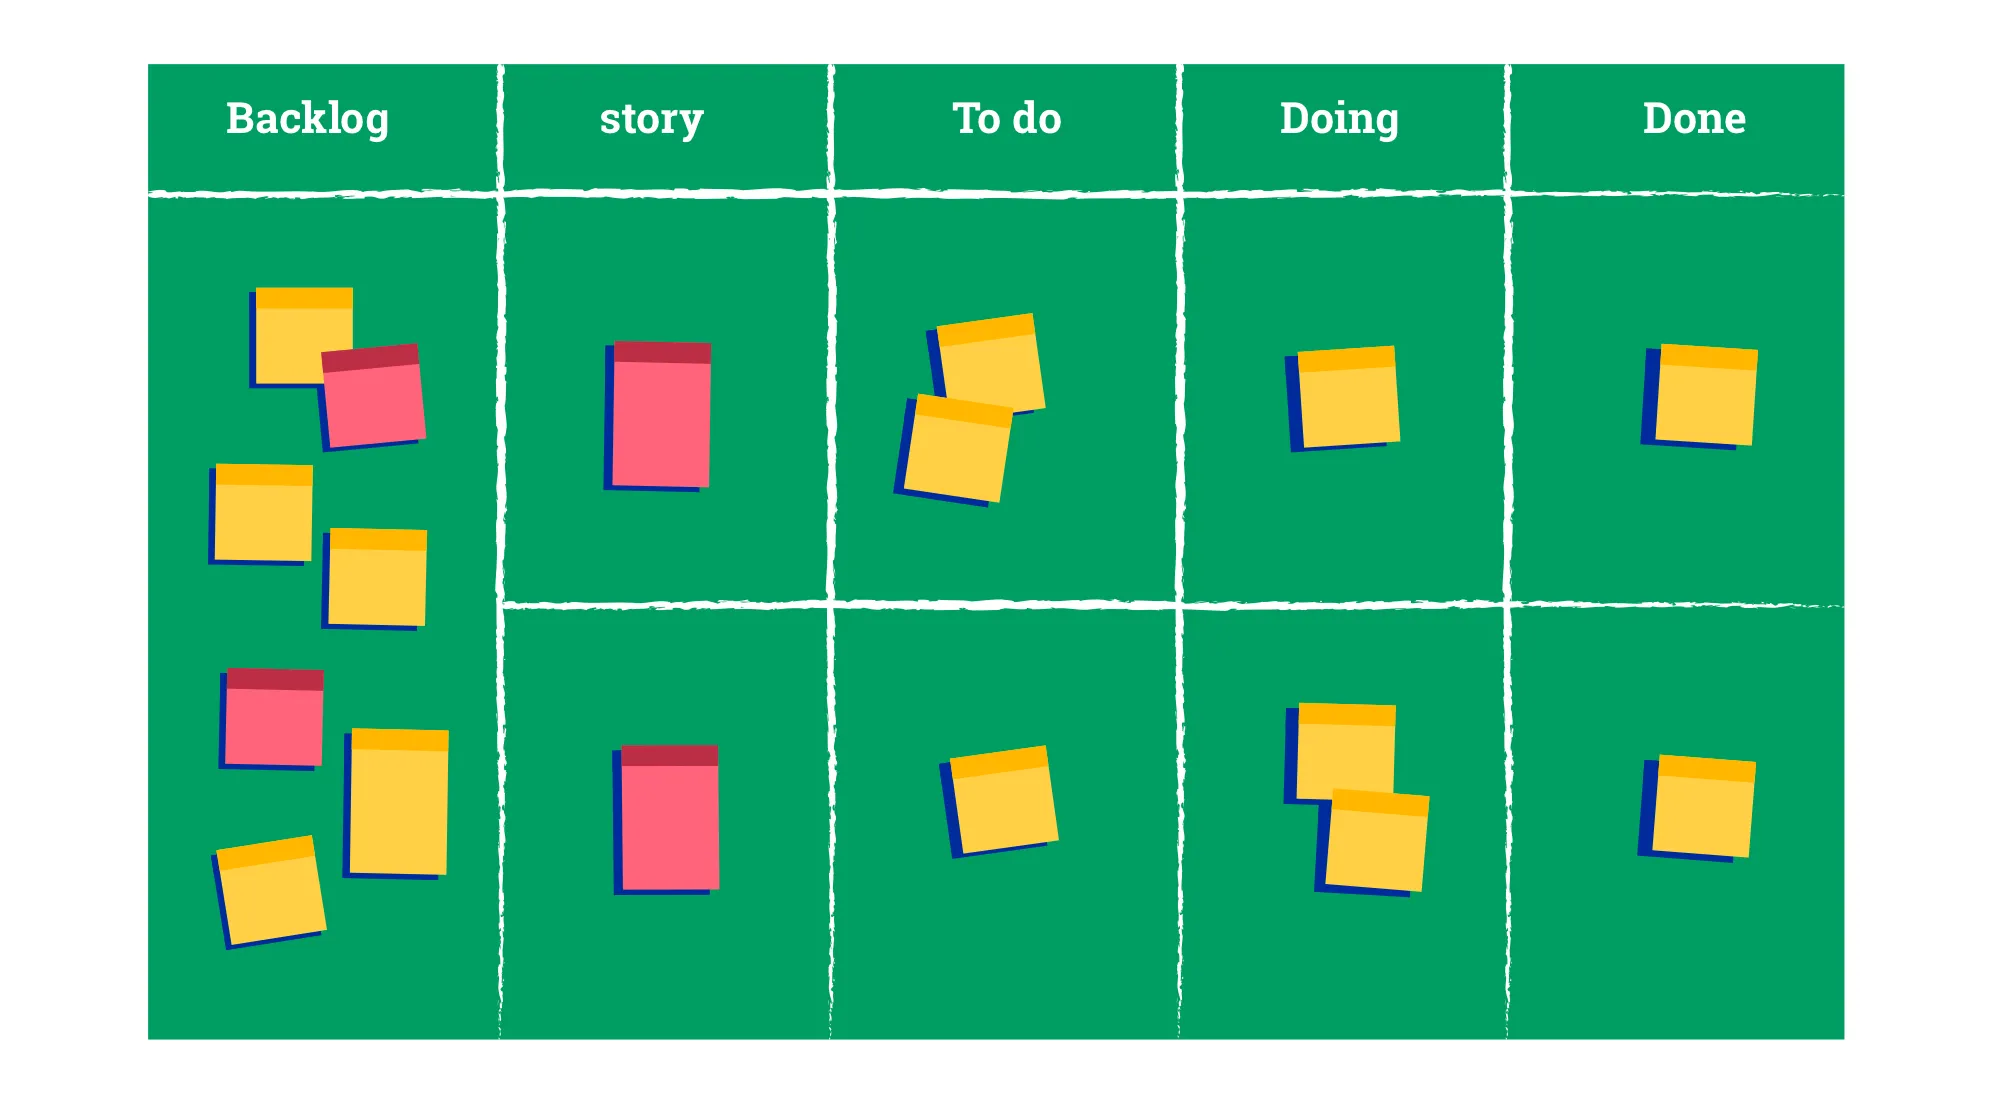
\includegraphics[width=0.8\columnwidth]{capitolo1/scrumb-board.png}
  \caption{Esempio di organizzazione delle attività nella Scrum Board}
  \textbf{Fonte}: \href{https://www.zoho.com/sprints/what-is-a-scrum-board.html}{https://www.zoho.com/sprints/what-is-a-scrum-board.html}
\end{figure}

Un altro evento fondamentale che fa parte di Scrum, al quale ho avuto modo di partecipare, è lo \textbf{\textit{sprint review}}. Quest'ultimo consiste in una riunione di fine sprint in cui si ispezionano i risultati dell'incremento insieme agli \textit{stakeholders}, decidendo eventuali cambiamenti da apportare al \textit{product backlog}. \\

\subsection{Manutenzione}
In seguito al rilascio di un \textit{software}, l'azienda si impegna a seguire la sua naturale evoluzione nel tempo, adattandolo sempre a nuove esigenze, e a risolvere eventuali errori. Per questo Sync Lab offre servizi di manutenzione che possono essere di tre tipi:
\begin{itemize}
  \item \textbf{Manutenzione correttiva}: permette di correggere eventuali difetti del prodotto;
  \item \textbf{Manutenzione adattiva}: permette di adattare il \textit{software} a cambiamenti dell'ambiente operativo;
  \item \textbf{Manutenzione evolutiva}: permette di estendere le funzionalità del prodotto esistente.
\end{itemize}